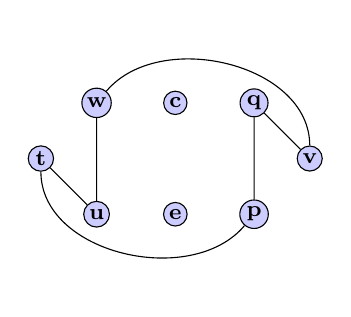
\begin{tikzpicture}
[node distance=1cm, xscale=.75, yscale=.75]
\node (w) [draw, circle, inner sep=1pt, fill=blue!20, font=\bfseries] {\footnotesize w};
\node (c) [draw, circle, inner sep=1pt, fill=blue!20, font=\bfseries, right of=w] {\footnotesize c};
\node (q) [draw, circle, inner sep=1pt, fill=blue!20, font=\bfseries, right of=c] {\footnotesize q};
\node (t) [draw, circle, inner sep=1pt, fill=blue!20, font=\bfseries, below left of =w] {\footnotesize t};
\node (v) [draw, circle, inner sep=1pt, fill=blue!20, font=\bfseries, below right of =q] {\footnotesize v};
\node (u) [draw, circle, inner sep=1pt, fill=blue!20, font=\bfseries, below right of=t] {\footnotesize u};
\node (p) [draw, circle, inner sep=1pt, fill=blue!20, font=\bfseries, below left of=v] {\footnotesize p};
\node (e) [draw, circle, inner sep=1pt, fill=blue!20, font=\bfseries, left of=p] {\footnotesize e};
\draw (t) to [out=-90, in=-130] (p);
\draw (w) to [out=50, in=90] (v);
\draw (p) -- (q) -- (v);
\draw (t) -- (u) -- (w);
\end{tikzpicture}
